\documentclass[a4paper,12pt]{article}
\usepackage[slovene]{babel}
\usepackage[utf8]{inputenc}
\usepackage[T1]{fontenc}
\usepackage{lmodern}
\usepackage{graphicx}
\usepackage{amsmath}
\pagenumbering{arabic}
\usepackage{wrapfig}
\usepackage{tabularx}
\usepackage[table]{xcolor}
\usepackage{amsfonts}
\usepackage{lipsum}
\usepackage{amsmath,amsthm}
\usepackage{ragged2e}
\usepackage{framed}
\usepackage{amssymb}
\usepackage{float}


\newtheorem{theorem}{Izrek}

\title{ \textbf{ Štetje rešitev klasičnega problema nahrbtnika} \\
  \large Poročilo pri predmetu Finančni praktikum}
\author{Kristina Vatovec in Žan Mikola}
\date{Januar 2021}

\begin{document}
\begin{titlepage}
\maketitle
\thispagestyle{empty}
\pagestyle{empty}
\end{titlepage}


\tableofcontents
\listoffigures

\newpage
\section{Uvod}

\noindent Napisano poročilo je sklepni del projektne naloge pri predmetu Finančni praktikum.
\vspace{3mm}

\noindent Projektna naloga se nanaša na problem štetja rešitev klasičnega problema nahrbtnika. Pri delu sva se oprla na članek Štefankovič idr. (2012).
\vspace{3mm}

\noindent V prvem delu poročila je opisan problem in predstavljen algoritma za dan problem.  Glavni del projektne naloge je bila implementacija algoritma v razdelku 2 . Algoritem sva napisala v programskem jeziku Python . 
\vspace{3mm}

\noindent Sledil je eksperimentalni del, kjer sva poskušala ugotoviti ali pri raličnih vhodnih podatkih prihaja do sprememb časovne zahtevnosti. Algoritem sva preizkusila pri različnem številu predmetov, poskusov in pa vrednostih epsilona.  Sklepi so povzeti v poglavju 3. 
\vspace{3mm}

\noindent 
Da bi bila izkušnja  reševanje problema za samega uporabnika bolj zanimiva sva v okviru projektne naloge dodala grafični uporabniški vmesnik. 


\newpage



\section{Opis problema}


Podanih je n elementov  z celoštevilskimi težami \(w_{1},...,w_{n}\) in kapaciteto C, ki je prav tako celo število  Privzemimo štetje klasičnega problema nahrbtnika.
S pomočjo algoritma, ki temelji na dinamičnem programiranju želimo poiskati oceno za  število rešitev problema znotraj relativne napake \(1 \pm \epsilon\)  v polinomskem času n in \(1/\epsilon\).
 
\vspace{3mm}
\noindent Preden nadaljujemo, omenimo naslednji izrek, ki je bistvenega pomena pri samem problemu.

 \begin{theorem}
Podane so teže \(w_{1},...,w_{n}\) in kapaciteta C pri problemu nahrbtnika. Naj bo Z število rešitev problema. Obstaja deterministični algoritem, ki za vsak \( \epsilon \in [0,1]\) vrne \(\uppercase{z}^{'} \)za katerega velja  
\( \uppercase{z} \leq \uppercase{z}^{'} \leq \uppercase{z}(1 + \epsilon) \) .
\end{theorem}


\noindent Poglejmo si še funkcijo $T : \{0, \ldots, n\} \times \{0, \ldots, s\} \rightarrow \mathbb{R}_{\geq 0} \cup \{\infty \}  $ , ki je definirana v spodnjem algoritmu.


\begin{framed}
Vhod: Celaštevila \(w_{1},...,w_{n}\), C in \( \epsilon > 0\).
\begin{enumerate}
\item Postavimo \(\uppercase{t}[0,0] = 0\) and \(\uppercase{t}[o,j] = \infty \) za \(j > 0\).
\item Postavimo \( \uppercase{q} = ( 1+ \epsilon/(n + 1))\) in \( s= \lceil n log_{\uppercase{q}}2 \rceil\).
\item Za \( i = 1 \to n\), za \( j = 0 \to s \), postavim

\[ 
\uppercase{t}[i, j]=\ min_{\alpha \in [0,1]} max \left\{
\begin{array}{ll}
      \uppercase{t}[i - 1, \lceil j + log_{\uppercase{q}}\alpha \rceil ], \\
      \uppercase{t}[i - 1, \lceil j + log_{\uppercase{q}}(1 - \alpha) \rceil ] + w_{i}, 
      
\end{array} 
\right. 
\]
kjer po dogovoru velja \( \uppercase{t}[i - 1, k] = 0 \) za \( k <0\).

\item Naj bo
\[
j^{'} := max\{j : \uppercase{t}[n, j] \leq \uppercase{C} \}.
\]
\item Izhod \(\uppercase{Z}^{'} := \uppercase{Q}^{j^{'} + 1} \)
\end{enumerate}
\end{framed}



\noindent Pri iskanju minimuna funkcije T v odvisnost od parametra $\alpha \in [0,1]$, je v resnici dovolj gledati le $\alpha$, ki ustrezajo vrednostim diskretne množice $S$. Za $ j \in \{0, 1, \ldots, s\}$, je množiča $S = S_{1} \cup S_{2}$, kjer $S_{1} = \{Q^{-j}, \ldots, Q^0\}$ in $S_{2} = \{1-Q^{0}, \ldots, 1- Q^{-j}\}$. \\
\vspace{3mm}\\
\noindent Izkaže se, da izhodni podatek \(\uppercase{z}^{'}\) zadošča zgoraj napisanem izreku, kar pa je tisto, kar si želimo pri algoritmu za naš problem.\\

\vspace{3mm}
\noindent V tem algoritmu smo uporabili funkcijo T, vendar na prvi pogled ni povsem jasno kaj pomeni vrednost, ki jo vrne. Fukcija  je T je torej aproksimacijska funkcija funkcije $\tau$.  Funkcija $\tau :  \{0, \ldots, n\} \times \mathbb{R}_{\geq 0}  \rightarrow \mathbb{R} \cup \{\pm \infty \} $, kjer $\tau (i,a )$ vrne najmanjši $C$, Pri katerem obstaja vsaj $a$ rešitev problema nahrbtnika z težami $ \omega_{1} \ldots \omega_{n}$ in kapaciteto $C$. Fukcijo $\tau$ ne znamo efektivno izračunati, zato definiramo fukcijo $T$. \\
 

\noindent Torej točno število rešitev problema nahrbtnika je $$Z= max\{a: \tau (n,a) \leq C\} $$

\newpage
\section{Algoritem}

\noindent Kot sva že omenila v uvodu, je bil glavni del projektne naloge implementacija zgornjega algitma.
\vspace{3mm}

\noindent Celotna kodo s kometarji  sva dodala na repozitorij. Napisana je v programskem jeziku \text{python}in jo  lahko poiščete v datoteki 
pod imenom \textit{program.py}.

\vspace{3mm}
\noindent Spodaj pa si lahko ogledate glavno fukncijo v sami kodi.

\vspace{5mm}
\begin{figure}[h]
\centering
\includegraphics[width=1.0\textwidth]{koda1}
\end{figure}


\newpage

\begin{figure}[h]
\centering
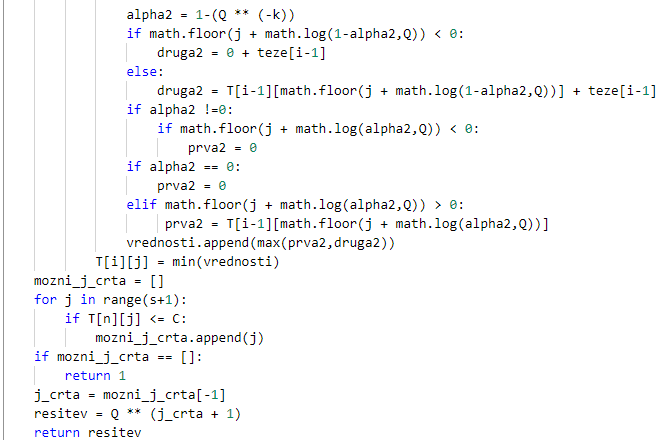
\includegraphics[width=1.0\textwidth]{koda2}
\end{figure}

\newpage

\section{Časovna zahtevnost in generirani podatki}

\noindent V eksperimentalnem delu  sva poskušala ugotoviti ali pri raličnih vhodnih podatkih prihaja do sprememb časovne zahtevnosti.  Bolj natančno, zanimala naju je hitrost izračunane rešitve  pri različnih vrendostih epsilona. 

\noindent Najprej sva sestavila kodo za generiranje podatkov, ki jo lahko najdete v datoteki \textit{program.py}.  Koda je napisana na način, da podatke na koncu shrani v excelovo datoteko.
\vspace {3mm}

\noindent Generirane podatkov lahko razdelimo v tri skupin in sicer glede na število predmetov, ki jih imamo v nahrbtniku.
\noindent V prvem nahrbtniku je 5 predmetov, v drugem 10 in v tretjem 20. Nato pa sva si izbrala nekaj vrednosti epsilonov in za vsako vrednost naredila 10 poskusov.
\vspace{3mm}

\noindent Ruzultati so v skladu s tem kar sva pričakovala. Bolj natančno kot želimo rešitev, torej manjši epislon kot si izberemo več časa je potrebnega.
\noindent Seveda pa čas narašča tudi z naraščanjem števila predmetov v nahrbtniku.
\vspace{3mm}

\noindent Rezultate so zbrani  v spodnjih grafih.

\newpage


\begin{figure}[H]
\centering
\caption{Eksperiment : 5 predmetov in 10 poskusov}
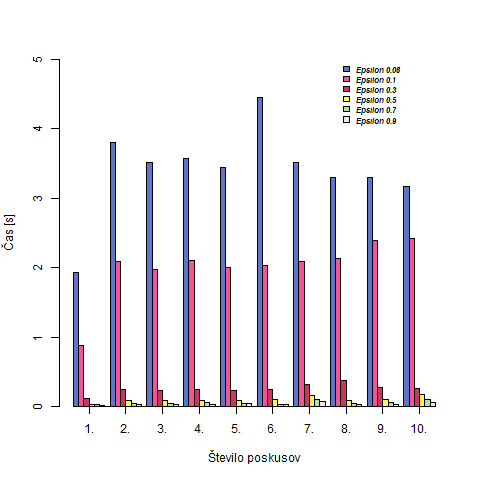
\includegraphics[width=10cm, height = 10cm]{5predmetov}
\end{figure}


\begin{figure}[H]
\centering
\caption{Eksperiment :10 predemtov in 10 poskusov}
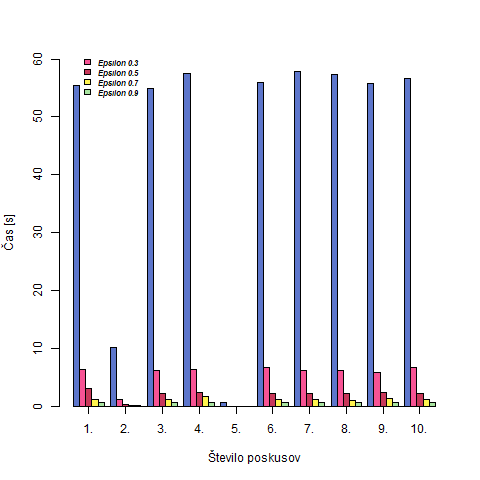
\includegraphics[width=11cm, height = 10cm]{10predmetov}
\end{figure}

\begin{figure}[H]
\centering
\caption{Eksperiment: 20 predmetov in 20 poskusov}
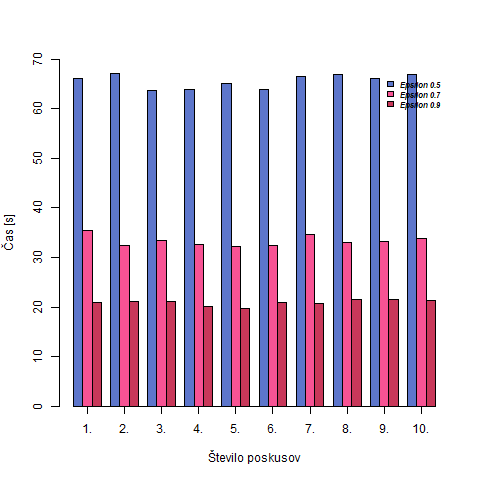
\includegraphics[width=10 cm, height = 10cm]{20predmetov}
\end{figure}



\newpage

\noindent V zadnjem delu eksperimentalnega dela pa sva še naredila primerjavo točnih vrednosti problema in pa izračunane približke števila rešitev in prišla do zanimive ugotovitve. 
\vspace{3mm}

\noindent V tem delu eksperimenta sva izbrala nahrbtnik 10 predmetov in nahrbtnik 20 predmetov. Rezultati so pokazali, da je odstopanje enako ne glede na teže predmetov v naboru desetih oziroma 20 predmetov. 
\vspace{5mm}

\begin{figure}[H]
\centering
\caption{Razlika med točno vrednostjo in približkom za 10 predmetov}
\includegraphics[width=11cm, height = 10cm]{Odstopanje10}
\end{figure}

\begin{figure}[H]
\centering
\caption{Razlika med točno vrednostjo in približkom za 20 predmetov}
\includegraphics[width=10 cm, height = 10cm]{Odstopanje20}
\end{figure}


\newpage

\section{Viri}

\begin{itemize}
\item Štefankovič, Vempala, Vigoda (2012). A deterministic polynomial time approximation scheme for counting knapsack solution.
\end{itemize}









\end{document}